\documentclass[../main.tex]{subfiles}
\begin{document}
\chapter{Homomorphisms}
\section{Homomorphisms}
Some groups are not literally (i.e. set-theoretically) \textit{equal} but, nevertheless \textit{share the same structure}.
For example $\Sym\{\text{Deck of Cards}\}$ and $\Sym\{\text{52 people}\}$.
\begin{definition}[Homomorphims]
  A \textit{homomorphism} is a map between groups, $\phi: G \to H$, that preserves the group structure, that is:
  \[
    \phi(g \cdot g') = \phi(g) * \phi(g')
  \]
  for all $g, g' \in G$. Where $\cdot$ is the binary operation on $G$ and $*$ is the binary operation on $H$.
\end{definition}
\begin{remark}[Notation]
  Usually differentiating the two binary operations is unnecessary if it is obvious which groups elements we are working with and the operation is fairly ``normal''.
\end{remark}
\begin{example}
  \begin{enumerate}
    \item For any two groups $G, H$ the map $\phi: G \to H$, $g \mapsto e_H$ is the \textit{trivial homomorphism}.
    \item If $H \leq G$ then the map $i: H \to G$, $h \mapsto h$ is the \textit{inclusion homomorphism}.
    \item Recall the group $C_n = \{z \in \C : z^{n} = 1\}$.
          If $n \mid m$ then the map $\phi: C_m \to C_n$, $z \mapsto z^{m/n}$ is a homomorphism.
          Since $n \mid m$, $m/n$ is an integer otherwise we could end up with multi-valued answers.
          \begin{align*}
            \phi\left(e^{\frac{2\pi i k}{m}} e^{\frac{2 \pi i l}{m}}\right) &= \phi\left(e^{\frac{2\pi i}{m}(k + l)}\right) \\
                                                                            &= e^{\frac{2\pi i}{m}(k + l)\cdot \frac{m}{n}} \\
                                                                            &= e^{\frac{2\pi}{n}(k + l)} \\
                                                                            &= \left(e^{\frac{2 \pi i k}{m}}\right)^{m/n} \left(e^{\frac{2 \pi i l}{m}}\right)^{m/n} \\
                                                                            &= \phi\left(e^{\frac{2\pi i k}{m}}\right) \phi\left(e^{\frac{2\pi i l}{m}}\right)
          \end{align*}
    \item Since $\det(AB) = \det(A)\det(B)$, the determinant function, $\det: \GL_2(\R) \to \R \setminus \{0\}$, $A \to \det(A)$ is a homomorphism.
          $\GL_2(\R)$ is the group of all $2\times2$ invertible real matrices, together with the operation of matrix multiplication.
  \end{enumerate}
\end{example}
\begin{proposition}
  If $\phi: G \to H$ is a homomorphism then:
  \begin{enumerate}
    \item $\phi(e_G) = e_H$.
    \item $\phi(g^{-1}) = \phi(g)^{-1}$ for all $g \in G$.
  \end{enumerate}
\end{proposition}
\begin{proof}
  \begin{enumerate}
    \item $\phi(e_G) \cdot \phi(e_G) = \phi(e_G \cdot e_G)$ since $\phi$ is a homomorphism.
      Thus $\phi(e_G) \cdot \phi(e_G) = \phi(e_G)$ so $\phi(e_G) = e_H$ by uniqueness of identities.
    \item $\phi(g) \cdot \phi(g^{-1}) = \phi(g \cdot g^{-1}) = \phi(e_G) = e_H$ so therefore $\phi(g^{-1}) = \phi(g)^{-1}$ by uniqueness of inverses.
  \end{enumerate}
\end{proof}
\section{Isomorphisms}
\begin{definition}[Isomorphism]
  If a homomorphism $\phi: G \to H$ is also a \textbf{bijection} then it is an \textit{isomorphism}. We write $G \cong H$.
\end{definition}
From the perspective of group theory, if $G \cong H$ then $G$ and $H$ are ``the same''.
\begin{example}
  \begin{enumerate}
    \item Recall $C_n = \{z \in \C : z^{n} = 1\}$ and $\Z_n = \{0, 1, \ldots, n - 1\}$ with operation $+_n$.

      Let $\phi: \Z_n \to C_n$, $k \mapsto e^{\frac{2\pi i k}{n}}$.
      Clearly $\phi$ is bijective as the solutions to $z^{n}$ are exactly $e^{\frac{2\pi i k}{n}}$ for $k = 0, 1, \cdots, n-1$.
      Furthermore, for any $k, l \in \Z_n$:
      \[
        k + l = np + (k +_n l)
      \]
      for some $p \in \Z$.

      To check that $\phi$ is an isomorphism:
      \begin{align*}
        \phi(k +_n l) &= e^{\frac{2 \pi i}{n}(k +_n l)} \text{ by definition of $\phi$}\\
                      &= e^{\frac{2 \pi i}{n}(np)} e^{\frac{2 \pi i}{n}(k +_n l)} \\
                      &= e^{\frac{2 \pi i}{n}(np + (k +_n l))} \\
                      &=e^{\frac{2 \pi i}{n}(k + l)} \\
                      &= e^{\frac{2 \pi i}{n} k} e^{\frac{2 \pi i}{n} l} \\
                      &= \phi(k) \phi(l) \text{ by definition of $\phi$}
      \end{align*}
      Thus $\phi$ is a homomorphism, and hence also an isomorphism.
      That is $\Z_n \cong C_n$ for all $n$.
    \item Consider the two groups $(\R, +, 0)$ and $(\R_{> 0}, \times, 1)$ with the map:
      \[
        \exp: (\R, +, 0) \to (\R_{> 0}, \times, 1) \text{ given by } x \mapsto e^{x}
      \]
      Since:
      \[
        \exp(x + y) = e^{x + y} = e^{x}e^{y} = \exp(x)\exp(y)
      \]
      so $\exp$ is a homomorphism.
      Since $\exp^{-1} = \ln$, $\exp$ is also a bijection, thus $\exp$ is an isomorphism.
      So $(\R, + , 0) \cong (\R_{>0}, \times, 1)$.
  \end{enumerate}
\end{example}
\begin{proposition}
  Some useful properties of homomorphisms and isomorphisms are:
  \begin{enumerate}
    \item If $\phi: G \to H$ is an isomorphism, so is $\phi^{-1}$.
    \item If $G \xrightarrow{\phi} H \xrightarrow{\psi} K$ are homomorphisms, so is $\psi \circ \phi$.
    \item $\cong$ is an equivalence relation.
  \end{enumerate}
\end{proposition}
\begin{proof}[\textbf{i}]
  $\phi$ is an isomorphism so is bijective, therefore $\phi^{-1}$ is also bijective.
  Consider $g_1, g_2 \in G$ and $h_1, h_2 \in H$ where $h_1 = \phi(g_1), h_2 = \phi(g_2)$:
  \begin{align*}
    \phi^{-1}(h_1) \cdot \phi^{-1}(h_2) &= g_1 \cdot g_2 \\
                                        &= \phi^{-1}(\phi(g_1 \cdot g_2)) \\
                                        &= \phi^{-1}(\phi(g_1)\phi(g_2)) \\
                                        &= \phi^{-1}(h_1 \cdot h_2)
  \end{align*}
  So $\phi^{-1}$ is also a homomorphism.
  Thus $\phi^{-1}$ is an isomorphism.
\end{proof}
\begin{proof}[\textbf{ii}]
  Let $g_1, g_2 \in G$:
  \begin{align*}
    (\psi \circ \phi)(g_1 \cdot g_2) &= \psi(\phi(g_1 \cdot g_2)) \\
                                     &= \psi(\phi(g_1) \cdot \phi(g_2)) \text{ as $\phi$ is a homomorphism} \\
                                     &= \psi(\phi(g_1)) \cdot \psi(\phi(g_2)) \text{ as $\psi$ is a homomorphism}\\
                                     &= (\psi \circ \phi)(g_1) \cdot (\psi \circ \phi)(g_2)
  \end{align*}
So $\psi \circ \phi$ is a homomorphism.
\end{proof}
\begin{proof}[\textbf{iii}]
  Consider groups $G, H, K$.
  We need to check the following properties of equivalence relations hold:
  \begin{itemize}
    \item \textbf{Reflexive -} Consider the function $\id_G: G \to G$, $a \mapsto a$.
      This is clearly bijection and $\id_A(a_1 \cdot a_2) = a_1 \cdot a_2 = \id_A(a_1) \cdot \id_A(a_2)$ so is an isomorphism.
      So $G \cong G$.
    \item \textbf{Symmetric -} If $G \cong H$ then there is a isomorphism $\phi: G \to H$.
      Then from \textbf{i} we have that $\phi^{-1}: H \to G$ is an isomorphism.
      So $H \cong G$.
    \item \textbf{Transitive -} If $G \cong H$ and $H \cong K$ then there is isomorphisms $\phi: G \to H$ and $\psi: H \to K$.
      From \textbf{ii} we know that $\psi \circ \phi: G \to K$ is a homomorphism.
      Since $\phi$ and $\psi$ are both bijective $\psi \circ \phi$ is also bijective.
      Thus $\psi \circ \phi$ is a isomorphism, so $G \cong K$.
  \end{itemize}
  All three requirements satisfied so $\cong$ is an equivalence relation.
\end{proof}
\begin{remark}
  $\cong$ being an equivalence relation is why two groups are considered ``the same'' when they are isomorphic.
\end{remark}
\section{Image and Kernel}
We saw earlier that every subgroup leads to an inclusion homomorphism.
The converse is also true.
That is, homomorphisms lead to subgroups.

\begin{definition}[Image]
  Let $\phi: G \to H$ be a homomorphism, then the image of $\phi$ is:
  \[
    \im(\phi) = \{h \in H : \exists g \in G \text{ s.t. } \phi(g) = h\}
  \]
\end{definition}
\begin{definition}[Kernel]
  Let $\phi: G \to H$ be a homomorphism, then the kernel of $\phi$ is:
  \[
    \ker(\phi) = \{g \in G: \phi(g) = e_H\}
  \]
\end{definition}
\begin{center}
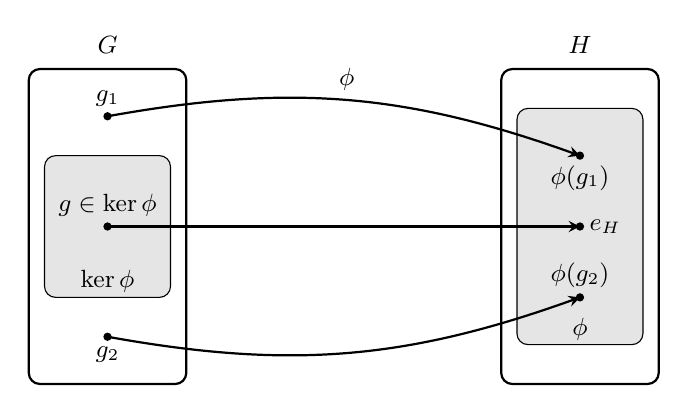
\begin{tikzpicture}[every node/.style={font=\small}, >=stealth]
\draw[rounded corners, thick] (-3,-2) rectangle (-1,2);
\draw[rounded corners, thick] (3,-2) rectangle (5,2);
\node at (-2,2.3) {$G$};
\node at (4,2.3) {$H$};

\draw[fill=gray!20, rounded corners] (-2.8,-0.9) rectangle (-1.2,0.9);
\node at (-2,-0.7) {$\ker \phi$};

\draw[fill=gray!20, rounded corners] (3.2,-1.5) rectangle (4.8,1.5);
\node at (4,-1.3) {$\im \phi$};

\coordinate (g1) at (-2, 1.4);
\coordinate (g2) at (-2, -1.4);
\coordinate (gker) at (-2, 0);
\coordinate (pg1) at (4, 0.9);
\coordinate (pg2) at (4, -0.9);
\coordinate (eh) at (4, 0);

\draw[->, thick] (g1) to[bend left=15] node[above] {$\phi$} (pg1);
\draw[->, thick] (gker) -- (eh);
\draw[->, thick] (g2) to[bend right=15] (pg2);

\fill (g1) circle (1.5pt) node[above] {$g_1$};
\fill (gker) circle (1.5pt) node[above] {$g \in \ker \phi$};
\fill (g2) circle (1.5pt) node[below] {$g_2$};

\fill (pg1) circle (1.5pt) node[below] {$\phi(g_1)$};
\fill (eh) circle (1.5pt) node[right] {$e_H$};
\fill (pg2) circle (1.5pt) node[above] {$\phi(g_2)$};
\end{tikzpicture}
\end{center}
\begin{proposition}
  If $\phi: G \to H$ is a homomorphism then:
  \begin{enumerate}
    \item $\im(\phi) \leq H$
    \item $\ker(\phi) \leq G$
  \end{enumerate}
\end{proposition}
\begin{proof}[\textbf{i}]
  \begin{itemize}
   \item \textbf{Identity -} $e_H = \phi(e_G) \in \im \phi$
   \item \textbf{Closure -} For $\phi(g_1), \phi(g_2) \in \im \phi$, $\phi(g_1) \cdot \phi(g_2) = \phi(g_1 \cdot g_2) \in \im \phi$
   \item \textbf{Inverses -} For all $g \in G$, $\phi(g)^{-1} = \phi(g^{-1}) \in \im \phi$
  \end{itemize}
  As $\im \phi \subseteq H$ and all axioms are satisfied, $\im \phi \leq H$.
\end{proof}
\begin{proof}[\textbf{ii}]
  \begin{itemize}
    \item \textbf{Identity -} $\phi(e_G) = e_H \implies e_G \in \ker \phi$
    \item \textbf{Closure -} For $g_1, g_2 \in \ker \phi$, $\phi(g_1 \cdot g_2) = \phi(g_1) \cdot \phi(g_2) = e_H \cdot e_H = e_H$ so $g_1 \cdot g_2 \in \ker \phi$
    \item \textbf{Inverses -} For $g \in \ker \phi$, $\phi(g^{-1}) = \phi(g)^{-1} = e^{-1}_{H} = e_H$ so $g^{-1} \in \ker \phi$
  \end{itemize}
  As $\ker \phi \subseteq G$ and all axioms are satisfied, $\ker \phi \leq G$.
\end{proof}
\begin{proposition}
  \label{surjectiveInjectiveProp}
  Let $\phi: G \to H$ be a homomorphism.
  \begin{enumerate}
    \item $\phi$ is \textit{surjective} if and only if $\im \phi = H$.
    \item $\phi$ is \textit{injective} if and only if $\ker \phi = 1_G = \{e_G\}$
  \end{enumerate}
\end{proposition}
\begin{proof}[\textbf{i}]
  By definition of surjectivity.
\end{proof}
\begin{proof}[\textbf{ii}]
  \begin{proofdirection}{Assume $\phi$ is injective}
    Then $\ker \phi = \phi^{-1}(\{e_H\})$ has 0 or 1 elements but must include $e_G$ so, $\ker \phi = 1_G$.
  \end{proofdirection}
  \begin{proofdirection}{Assume $\ker \phi = 1_G$}
    If $\phi(g_1) = \phi(g_2)$ then $\phi(g_1 g^{-1}_{2}) = \phi(g_1)\phi(g_2)^{-1} = e_H$.
    So $g_1 g^{-1}_{2} \in \ker \phi$ so $g_1 g^{-1}_{2} = e_G$.
    Thus $g_1 = g_2$.
    Therefore $\phi(g_1) = \phi(g_2) \implies g_1 = g_2$ so $\phi$ is injective.
  \end{proofdirection}
\end{proof}
\begin{proposition}
  A homomorphism $\phi: G \to H$ is an isomorphism if and only if $\im \phi = H$ and $\ker \phi = 1_G$
\end{proposition}
\begin{proof}
  Combine \textbf{i} and \textbf{ii} in \cref{surjectiveInjectiveProp} above.
\end{proof}
\section{Cyclic Groups}
The groups $C_n \cong \Z_n$ that we described above have a special property:
\begin{definition}[Cylic Group]
  A group $G$ is \textit{cyclic} if there exists an element $g \in G$ such that:
  \[
    G = \{g^{k} : k \in \Z\}
  \]
  That is $G = \langle g \rangle$ where $g$ is called a \textit{generator} of $G$.
\end{definition}
\begin{example}
  \begin{enumerate}
    \item $C_n \{z \in \C: z^{n} = 1\}$ is cyclic with generator $e^{\frac{2\pi i}{n}}$.
    \item $\Z$ is cyclic with generator 1.
    \item $\Z_n$ is cyclic, since $\Z_n \cong C_n$.
  \end{enumerate}
\end{example}
\begin{theorem}
  If $G$ is cyclic then either:
  \begin{itemize}
    \item $G \cong C_n$ for some $n$
    \item $G \cong \Z$
  \end{itemize}
\end{theorem}
\begin{proof}
  Let $G$ be a cyclic group with generator $g$.
  Let
  \[
    S = \{k \in \N_0 : g^{k} = e\}\text{ and }
    n = \begin{cases}
    \min S & \text{ if } S \neq \emptyset \\
    \infty & \text{ if } S = \emptyset
    \end{cases}
  \]
  \begin{proofcases}
    \begin{case}{$n = \infty,\ S = \emptyset$}
      Define $\phi: \Z \to G$, $k \to g^{k}$.
      We now need to show that $\phi$ is an isomorphism.

      Since:
      \[
        \phi(k + l) = g^{k + l} = g^{k}g^{l} = \phi(k)\phi(l)
      \]
      so $\phi$ is a homomorphism.

      We know that $\phi$ is surjective since $G$ is cyclic so by definition $g^{k}$ $k \in \Z$ are the elements of $G$.

      To prove that $\phi$ is injective we need to show that $\ker \phi = \{0\}$.
      Suppose we have $k \in \ker \phi$ but $k \neq 0$.
      Since $\ker \phi \leq \Z$ we may replace $k$ by $-k$ if necessary and assume $k > 0$.
      $k \in \ker \phi$ so $\phi(k) = g^{k} = e$ and so $k \in S$.
      But then $S \neq \emptyset$ which is a contradiction.
      So we cannot have any elements in $\ker \phi$ that are not 0 and $0 \in \ker \phi$ since it is a homomorphism.
      Thus $\ker(\phi) = \{0\}$ so $\phi$ is an isomorphism.
    \end{case}
    \begin{case}{$n < \infty,\ S \neq \emptyset$}
      Define $\phi: \Z_n \to G$, $k \to g^{k}$.
      Since $k + l = qn + (k +_n l)$ and $g^{n} = e$ as $n \in S$:
      \[
        \phi(k)\phi(l) = g^{k}g^{l} = g^{k + l} = g^{qn + (k +_n l)} = (g^{n})^{q} g^{k +_n l} = g^{k +_n l} = \phi(k +_n l)
      \]
      so $\phi$ is a homomorphism.

      To prove surjectivity, since $G$ is cyclic, every element can be written as $g^{k}$ for some $k \in \Z$.
      Applying the division algorithm gives $k = nq + r$ for some $q \in \Z$ and $r \in \Z_n$
      Therefore:
      \[
        g^{k} = g^{nq + r} = (g^{n})^{q}g^{r} = g^{r} = \phi(r)
      \]
      so $\phi$ is surjective.

      To prove injectivity, suppose $k \in \ker \phi$, that is, $\phi(k) = g^{k} = e$ for some $k \in \Z_n$.
      So $k \in S$ and $0 \leq k < n$.
      Since $n$ was minimal in $S$ and we required that elements of $S$ are positive, it follows that $k = 0$.
      Thus $\ker \phi = \{0\}$ so $\phi$ is injective.
      Therefore $\phi$ is an isomorphism so $G \cong \Z_n \cong C_n$.
    \end{case}
  \end{proofcases}
\end{proof}
\begin{remark}[Notation]
  Because of this theorem we will write $C_n$ for \textbf{any} cyclic group of order $n$ (as all cyclic groups of equal order are isomorphic), and also $C_{\infty} \cong \Z$.
\end{remark}
\subsection{Element Order}
We can now define the order of an element in a group:
\begin{definition}[Element Order]
  For any group $G$, and element $g \in G$, let:
  \[
    \langle g \rangle = \{g^{k} : k \in \Z\} \leq G
  \]
  Note that $\langle g \rangle$ is cyclic so $\langle g \rangle \cong C_n$ for some $n \in \N_0 \cup \{\infty\}$.
  Then $n$ is the \textit{order} of $g$ and is denoted by $o(g)$ or $|g|$.
\end{definition}
Intuitively this is the smallest $n \in \N$ such that $g^{n} = e$ and if no such $n$ exists then the order of $g$ is infinite.
\section{Dihedral Groups Revisited}
Whenever $x, y \in G$ satisfy the dihedral relation $xy = yx^{-1}$, then for any $l > 0$:
\begin{align*}
  yx^{-l} &= (yx^{-1}) x^{1-l} \\
          &= xyx^{1-l} \\
          &= x(yx^{-1})x^{2-l} \\
          &= x^2yx^{2-l} \\
          &\;\; \vdots \text{ by induction}\\
          &= x^{l}y
\end{align*}

If $y^2 = e$, we also have:
\[
  yx^{l} = y(x^{l}y)y = y(yx^{-l})y=x^{-l}y
\]
In summary, $yx^{l} = x^{-l}y$ for any $l \in \Z$ provided $xy = yx^{-1}$ and $y^2 = e$.
\begin{remark}[Memorisation]
  This is almost like we can ``push'' the $x$ across the $y$ provided we swap the sign of the power.
\end{remark}
\begin{lemma}
  \label{dihedralLemma}
  Let $G$ be a group and $a, b \in G$, such that:
  \begin{itemize}
    \item $a^{n} = e$ for some $n \geq 3$
    \item $b^2 = e$
    \item $ab = ba^{-1}$
  \end{itemize}
  Then $\phi(r^{k}) = a^{k}$, $\phi(r^{k}s) = a^{k}b$ defines a homomorphism $\phi: D_{2n} \to G$ sending $r \mapsto a$ and $s \mapsto b$.
\end{lemma}
\begin{proof}
  There are two different forms of elements in $D_{2n}$, $r^{k}$ and $r^{k}s$, so there is a total of four cases to check each of the combinations:
  \begin{proofcases}
    \begin{case}{$r^{k},\ r^{l}$}
      \vspace{-2em}
      \begin{align*}
        \phi(r^{k})\phi(r^{l}) &= a^{k}a^{l} \\
                               &= a^{k + l} \\
                               &= a^{k +_n l} \text{ (as $a^{n} = e$)}\\
                               &= \phi(r^{k + l})
      \end{align*}
    \end{case}
    \begin{case}{$r^{k},\ r^{l}s$}
      \vspace{-2em}
      \begin{align*}
        \phi(r^{k})\phi(r^{l}s) &= a^{k} a^{l} b \\
                                &= a^{k + l} b \\
                                &= a^{k +_n l} b \\
                                &= \phi(r^{k + l}s) \\
                                &= \phi(r^{k} r^{l} s)
      \end{align*}
    \end{case}
    \begin{case}{$r^{k}s,\ r^{l}$}
      \vspace{-2em}
      \begin{align*}
        \phi(r^{k}s)\phi(r^{l}) &= a^{k} b a^{l} \\
                                &= a^{k - l} b \text{ (as $ba^{l} = a^{-l}b$)}\\
                                &= \phi(r^{k - l} s) \\
                                &= \phi(r^{k}s r^{l}) \text{ (as $r^{-l}s = sr^{l}$)}
      \end{align*}
    \end{case}
    \begin{case}{$r^{k}s,\ r^{l}s$}
      \vspace{-2em}
      \begin{align*}
        \phi(r^{k}s)\phi(r^{l}s) &= a^{k} b a^{l}b \\
                                 &= a^{k - l} b^2 \text{ (as $ba^{l} = a^{-l}b$)}\\
                                 &= a^{k - l} \text{ (as $b^2 = e$)}\\
                                 &= \phi(r^{k - l}) \\
                                 &= \phi(r^{k - l} s s) \text{ (as $s^2 = e$)}\\
                                 &= \phi(r^{k} s r^{l} s) \text{ (as $r^{-l}s = sr^{l}$)}
      \end{align*}
    \end{case}
  \end{proofcases}
  So in all possible cases $\phi$ is a homomorphism.
\end{proof}
\begin{proposition}
  Suppose $G$ has generating set $\{a, b\}$ such that:
  \begin{itemize}
    \item $a^{n} = e$
    \item $b^{2} = e$
    \item $ab = ba^{-1}$ (Dihedral relation)
    \item $|G| = 2n$
  \end{itemize}
  Then $G \cong D_{2n}$
\end{proposition}
\begin{proof}
  By \cref{dihedralLemma} there is a homomorphism $\phi: D_{2n} \to G$, $r \mapsto a$, $s \mapsto b$.

  Since $a$ and $b$ generate $G$, $\phi$ is surjective.

  We also have that $|D_{2n}| = 2n = |G|$.
  So $\phi$ is a surjection between two finite sets of equal size so must be bijective.

  Therefore $\phi$ is an isomorphism, thus $G \cong D_{2n}$.
\end{proof}
\end{document}
